\newcommand\myarrow{%
  \tikz\draw[thick,->] (0,0) -- ++(0,-1.1);
}

\chapter{矩阵与线性映射}
\begin{center}
	% \textcolor[RGB]{255, 0, 0}{\faHeart}所以生命啊,它苦涩如歌.\textcolor[RGB]{255, 0, 0}{\faHeart}
	「所以生命啊,它苦涩如歌」
\end{center}
\rightline{——《我用什么把你留住》}
\vspace{-5pt}
\begin{center}
	\pgfornament[width=0.36\linewidth,color=lsp]{88}
\end{center}

\section{线性方程组与矩阵}

\subsection{向量的矩阵表示}

这是一个前置知识,只需要读者记住即可,向量的矩阵表示是将向量竖起来写。

\begin{definition}{向量的矩阵表示}
	设向量$x\in \mathbb{F}^n$,$x=(x_1,x_2,x_3,\cdots,x_n)$的矩阵表示是$$\begin{pmatrix}  
		x_1 \\  
		x_2 \\
		x_3 \\
		\vdots \\
		x_n
	  \end{pmatrix} 
	$$记作$\boldsymbol{x}$\footnote{今后我们表示矩阵使用粗体的字母}或$\mathcal{M}(x)$;而矩阵的向量表示则表示为$\mathcal{V}(\boldsymbol{x})$,因此,满足下面的等式$$\boldsymbol{x}=\mathcal{M}(x);x=\mathcal{V}(\boldsymbol{x})$$
\end{definition}

则该$n\times 1$的矩阵也有相关的运算法则,分别为矩阵和与标量积,类比向量进行相关运算后竖着写则其表示形式,这里不再重复赘述相关性质,读者可根据章节\ref{sec:vector.operator}来自行证明,下面给出相关定义:

\begin{definition}{$n\times 1$矩阵的加法}
	若矩阵$\mathbf{A},\mathbf{B}$同为$n\times 1$矩阵,其中$\mathbf{A}=\begin{pmatrix}  
		x_1 \\  
		x_2 \\
		x_3 \\
		\vdots \\
		x_n  
	  \end{pmatrix},\mathbf{B}=\begin{pmatrix}  
		y_1 \\  
		y_2 \\
		y_3 \\
		\vdots \\
		y_n  
	  \end{pmatrix}  $则$\mathbf{A}+\mathbf{B}$定义为$$\mathbf{A}+\mathbf{B}:=\begin{pmatrix}  
		x_1+y_1 \\  
		x_2+y_2 \\
		x_3+y_2 \\
		\vdots \\
		x_n+y_n  
		\end{pmatrix}$$
\end{definition}

同样的道理我们定义乘法

\begin{definition}{$n\times 1$矩阵的标量乘法}
	若标量 $\lambda\in \mathbb{F}$,其对一个$n\times 1$矩阵 $\boldsymbol{x} = \begin{pmatrix}  
		x_1 \\  
		x_2 \\
		x_3 \\
		\vdots \\
		x_n  
		\end{pmatrix}$ 的乘积定义为$$\lambda\boldsymbol{x}:=\begin{pmatrix}  
				\lambda x_1 \\  
				\lambda x_2 \\
				\lambda x_3 \\
				\vdots \\
				\lambda x_n  
				\end{pmatrix}$$
\end{definition}

\subsection{线性方程组与平面上的线性变换}

回顾初中所学的一些内容,我们了解到了二元一次方程组,它们形如:
$$\left\{\begin{matrix} 
	a_1x+b_1y=c_1 \\  
	a_2x+b_2y=c_2
  \end{matrix}\right. $$
这就是线性方程组的一种,通常可用于平面上的线性变换,下面一种情况就是平面上的线性变换:

\begin{figure}[htbp]
	\centering
	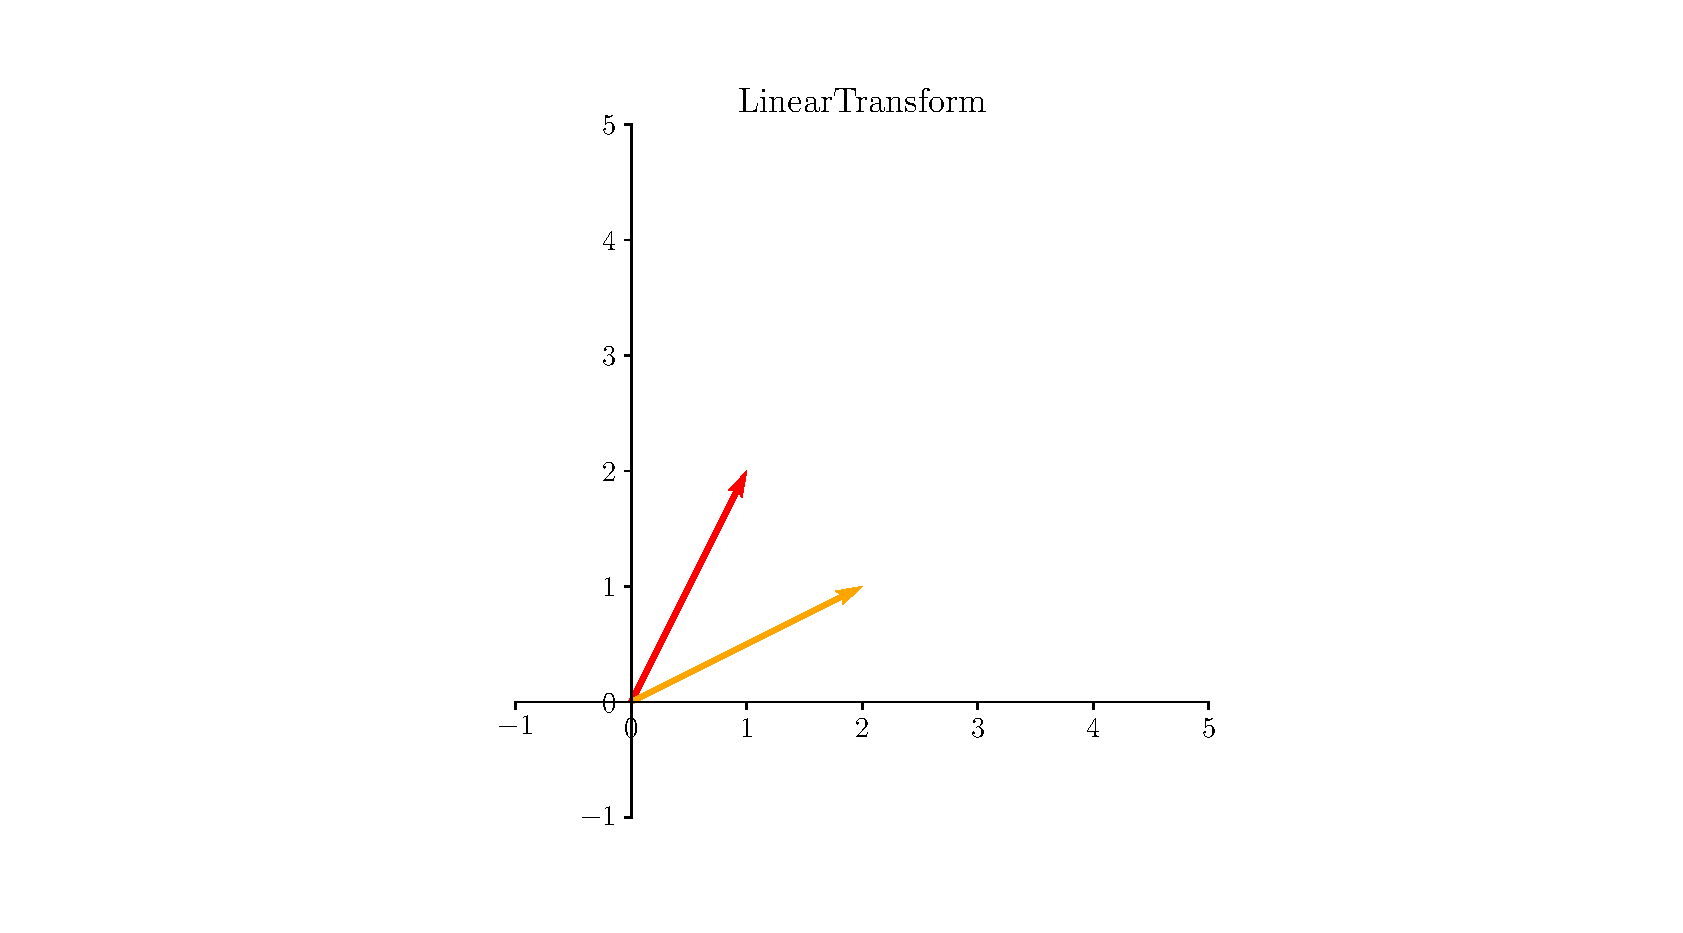
\includegraphics[width=0.7\linewidth]{figure/eps/LinearTransform.eps}
	\caption{线性变换}
	\label{fig:LinearTransform}
\end{figure}

我们平常所使用的坐标系是直角坐标系,表示向量使用标准基$\left\{ (1,0),(0,1) \right\}$,所谓的线性变换是指如果将坐标系进行一个变化,使得构成这个系的基由原来的$\left\{ (1,0),(0,1) \right\}$变化成$\left\{ (x_1,y_1),(x_2,y_2) \right\}$后所表示的向量在原坐标系中所表示的坐标。如图\ref{fig:LinearTransform}所示,如果我们的基由原来的$\left\{ (1,0),(0,1) \right\}$变化成$\left\{ (1,2),(2,1) \right\}$,那么变换前坐标$(4,5)$的线性组合是$(4,5)=4(1,0)+5(0,1)$,而变化基后的坐标则变为$(14,13)=4(1,2)+5(2,1)$,即空间内的每一点$(x,y)=x(1,0)+y(0,1)$都变化为$(x+2y,2x+y)=x(1,2)+y(2,1)$,设变化后的空间的每一个点在原坐标系的坐标表示为$(x',y')$;表示为线性方程组就是$$\left\{\begin{matrix} 
	1x+2y=x' \\  
	2x+1y=y'
  \end{matrix}\right. $$如果我们把这个式子进一步抽象,可以得到一个矩阵方程\begin{equation}
	\begin{pmatrix}  
	1 & 2 \\  
	2 & 1  
  \end{pmatrix} \begin{pmatrix}  
	x \\  
	y  
  \end{pmatrix} =\begin{pmatrix}  
	x' \\  
	y'  
  \end{pmatrix}
  \label{eq:MatrixIntro}
\end{equation}

\begin{example}
	\label{exam:scale}
	在平面直角坐标系中,向量$a=\overrightarrow{OP_1}=(3,2),b=\overrightarrow{OP_2}=(4,7)$;
	\begin{enumerate}
		\item 求$\triangle OP_1P_2$的面积;
		\item 若将$x$轴的每一个值扩大一倍,求标准基经过变换后的向量集合;
		\item 若将$y$轴的每一个值扩大一倍,求变换后的三角形面积$\triangle OP_1'P_2'$
	\end{enumerate}
	\tcblower
	\textcolor{purple}{\textbf{解}}:
	\begin{enumerate}
		\item 可使用割补法和叉积法,对于割补法,如图\ref{fig:source.gb}所示,则是将其填充为矩形,即$S=4\times 7-S_1-S_2-S_3$其中$S_1=4\times 7\div 2=14,S_2=(2+7)\times 1 \div 2=4.5,S_3=2\times 3 \div 2 =3$则$\triangle OP_1P_2$的结果为$S=28-14-18-3=6.5$,若使用叉积法,则有公式$$S=\frac{1}{2}\left| x_1y_2-x_2y_1 \right|=\frac{1}{2}=\left| 3\times 7-2\times 4 \right|=6.5$$
		\item $\left\{ (2,0),(0,1) \right\}$
		\item 若$y$轴扩大一倍,则该部分所有的面积都扩大一倍,所以$6.5\times 2=13$
	\end{enumerate}
\end{example}

\begin{figure}[htbp]    % 常规操作\begin{figure}开头说明插入图片
	% 后面跟着的[htbp]是图片在文档中放置的位置, 也称为浮动体的位置, 关于这个我们后面的文章会聊聊, 现在不管, 照写就是了
	\centering            % 前面说过, 图片放置在中间
	\subfloat[三角形$\triangle OP_1P_2$图]   % 第一张子图的下标(注意: 注释要写在[]中括号内)
	{
		\label{fig:source}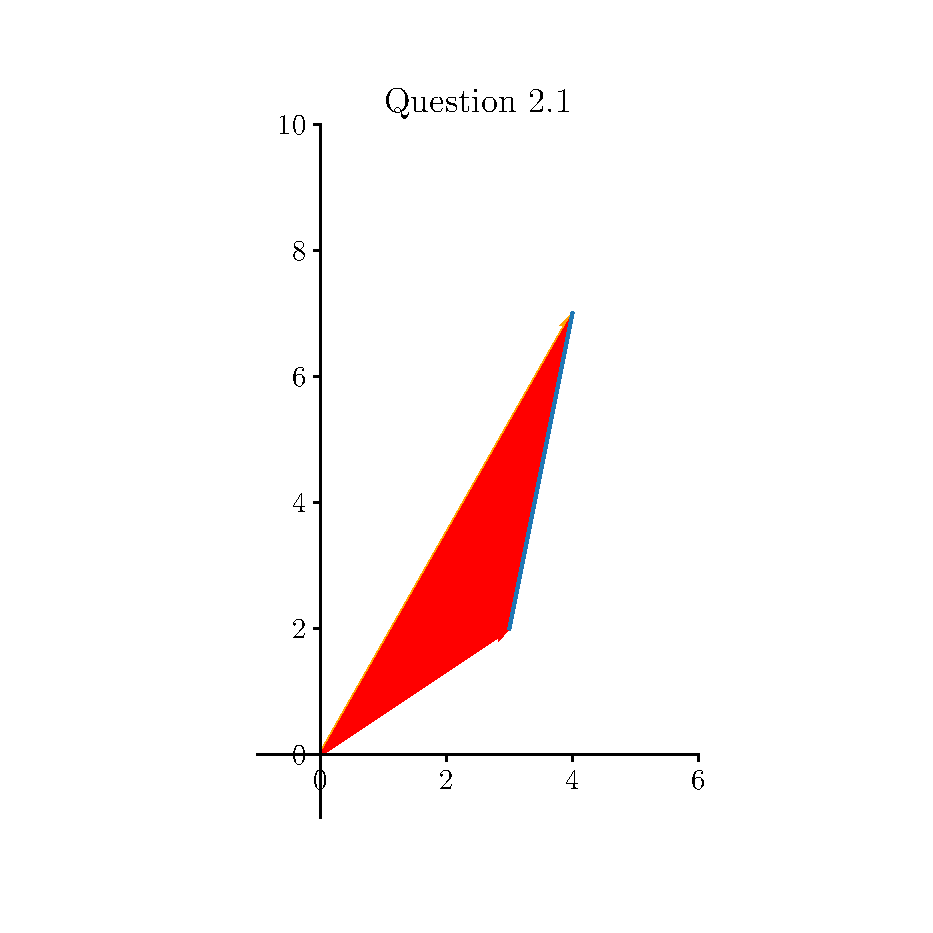
\includegraphics[width=0.5\textwidth]{eps/q21.eps}
		% \label{}命令为每个子图添加标签, 方便在正文中引用. 如果你不需要引用的话, 也可以不加这个命令, 写法在下面有: 
		% \label{}命令的{}内第一个{}中的内容fig:subfig1就是你插入的这张子图的标签, 注意每个标签都不能一样, 要用合适的编号去区分, 比如1, 2, 3......
		% \label{}命令中{}内\includegraphics[]{}就是真正插入图片的命令, []中的是图片的一些参数, {}就是图片的相对路径
		% width=0.4\textwidth 就是设置图片的大小, 这里设置的是文档宽度(\textwidth)的0.4倍, 在设置时注意不要超宽, 不然会报错, 大家多设置几个数尝试一下就能理解了
	}
	\subfloat[割补法]
	{
		\label{fig:source.gb}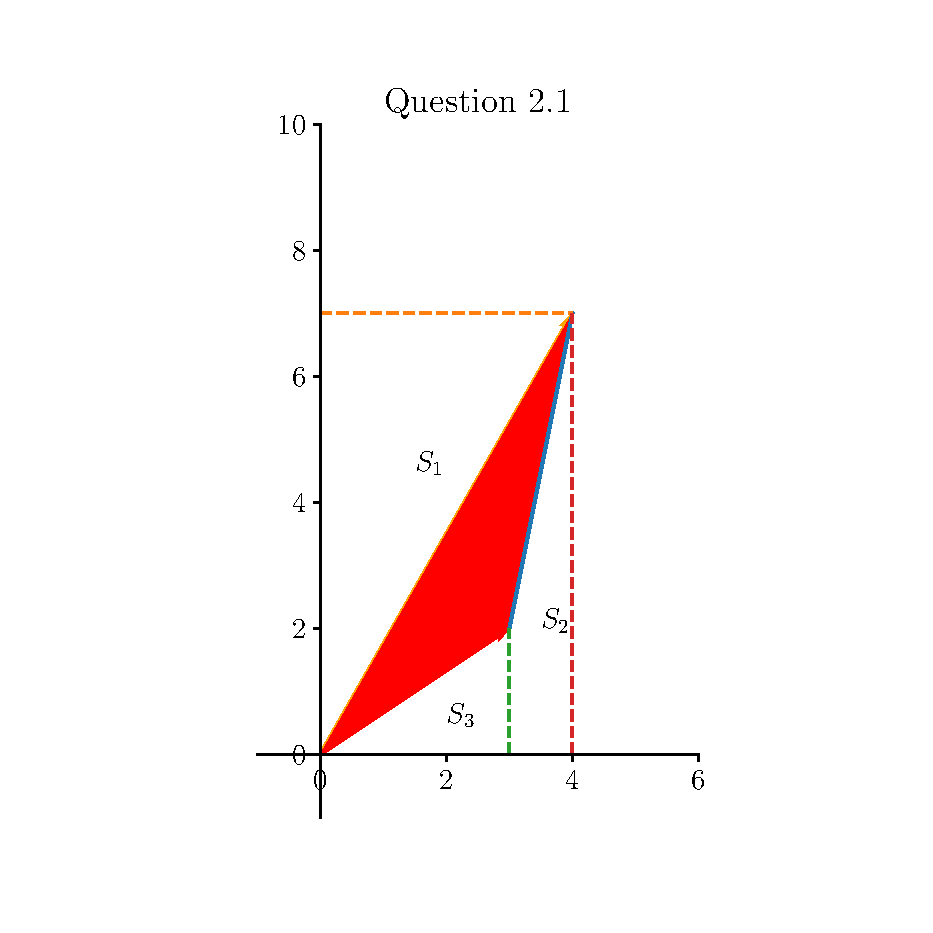
\includegraphics[width=0.5\textwidth]{eps/q21_gb.eps}
	}
	\caption{例题 2.1 图像}    % 整个图片的说明, 注释写在{}内
	\label{fig:pic.21}            % 整个图片的标签编号, 注意这里跟子图是一样的道理, 标签不能重复 
\end{figure}

为了方便表示,我们把公式\ref{eq:MatrixIntro}乘式中最左边的内容提取出来,称作变化矩阵,这个例子将是我们以后研究矩阵的一个特殊情况;为了方便描述,我们将该矩阵用$\mathbf{A}$表示
$$\mathbf{A}=\begin{pmatrix}  
	1 & 2 \\  
	2 & 1  
  \end{pmatrix}$$

若使用$\boldsymbol{x}$和$\boldsymbol{x'}$分别表示$(x,y)$和$(x',y')$的矩阵形式,那么公式\ref{eq:MatrixIntro}可表示为$$\boldsymbol{x'}=\mathbf{A}\boldsymbol{x}$$

接下来我们将矩阵$\mathbf{A}$中的第$i$行第$j$列元素表示为$\mathbf{A}_{i,j}$,例如$A_{1,2}=2$。

通过上面的描述,虽然我们并没有严格证明,但是我们也可以得知线性空间经过线性变换后,其结果仍然是线性空间。我们还是从二维平面出发来讲解矩阵的相关性质,于是我们有如下推论:

\begin{corollary}
	在二维平面内,矩阵$\mathbf{A}$表示其空间内的线性变换,设$x,y \in \mathbb{R}^2$且其矩阵表示分别为$\boldsymbol{x},\boldsymbol{y}$,则有如下推论:
	\begin{enumerate}
		\item $\mathbf{A}(\boldsymbol{x}+\boldsymbol{y})=\mathbf{A}\boldsymbol{x}+\mathbf{A}\boldsymbol{y}$
		\item 若$\lambda \in \mathbb{R}$则有$\lambda (\mathbf{A}\boldsymbol{x})=\mathbf{A}(c\boldsymbol{x})$
	\end{enumerate}
\end{corollary}

\begin{proof}
	\begin{enumerate}
		\item 设$x=(x_1,y_1),y=(x_2,y_2)$,则对于等式左侧$x+y=(x_1+x_2,y_1+y_2)$,其矩阵表示为$\begin{pmatrix}  
			x_1+y_1 \\  
			x_2+y_2  
		  \end{pmatrix} $,设$2\times 2$矩阵$\mathbf{A}$,令$$\mathbf{A}=\begin{pmatrix}  
			a & b \\  
			c & d  
		  \end{pmatrix} ,a,b,c,d \in \mathbb{R}$$那么类比矩阵方程\ref{eq:MatrixIntro},设结果向量为$(x',y')$我们可得矩阵式$$\begin{pmatrix}  
			a & b \\  
			c & d  
		  \end{pmatrix} \begin{pmatrix}  
			x_1+y_1 \\  
			x_2+y_2  
		  \end{pmatrix} $$的方程组式为$$\left\{\begin{matrix} 
			x'=a(x_1+y_1)+b(x_2+y_2) \\  
			y'=c(x_1+y_1)+d(x_2+y_2)
		  \end{matrix}\right. $$而根据标量加法分配法则,方程组可写成\begin{equation}\left\{\begin{matrix} 
			x'=ax_1+ay_1+bx_2+by_2 \\  
			y'=cx_1+cy_1+dx_2+dy_2
		  \end{matrix}\right. \label{eq:eqarray}\end{equation}同理右侧可表示为方程组式\ref{eq:eqarray},等式成立。$\square$
		\item 读者自证
	\end{enumerate}
\end{proof}

\subsection{矩阵表示线性方程组}

首先讲解什么是线性方程组,定义如下:

\begin{definition}{线性方程组}
	线性方程组是由多个线性方程组成的集合,通常表示为$$\begin{cases}
		a_{11}x_1 + a_{12}x_2 + \cdots + a_{1n}x_n = b_1 \\
		a_{21}x_1 + a_{22}x_2 + \cdots + a_{2n}x_n = b_2 \\
		\vdots \\
		a_{m1}x_1 + a_{m2}x_2 + \cdots + a_{mn}x_n = b_m
		\end{cases}$$
		其中,$ x_1, x_2, \ldots, x_n $ 是未知数,$ a_{ij} $ 是系数,$ b_i $ 是常数项。
\end{definition}

根据上面的矩阵式\ref{eq:MatrixIntro}所表示的二元一次方程组的几何意义,同样这里也可以看作是$n$维向量$x=(x_1,x_2,\\x_3,\cdots,x_n)$经过一个复杂的变化$\mathbf{A}$变为$b=(b_1,b_2,b_3,\cdots,b_n)$一样,所以同样我们可以将线性方程组的一般形式抽象成一个矩阵:$$\mathbf{A} \boldsymbol{x} = \boldsymbol{b}$$其中$$\mathbf{A} = \begin{pmatrix}
	a_{11} & a_{12} & \cdots & a_{1n} \\
	a_{21} & a_{22} & \cdots & a_{2n} \\
	\vdots & \vdots & \ddots & \vdots \\
	a_{m1} & a_{m2} & \cdots & a_{mn}
	\end{pmatrix},\boldsymbol{x}=\begin{pmatrix}
		x_1 \\
		x_2 \\
		\vdots \\
		x_n
		\end{pmatrix},\boldsymbol{b}=\begin{pmatrix}
			b_1 \\
			b_2 \\
			\vdots \\
			b_m
			\end{pmatrix}$$

\subsection{矩阵的定义}

我们已经对矩阵有了一个较为感性的认知,终于我们来到了系统讲解矩阵的这一部分,不过可能会让读者失望的是,矩阵的定义并非是你之前所认识的那样,是一个表示线性变换的符号;事实上,矩阵的真正定义其实就是一堆数字按照$m\times n$的方式排列而已,下面我们给出矩阵的定义。

\begin{definition}{矩阵的定义}
	矩阵是一个由圆括号\footnote{在一些教材中,会使用方形括号表示}包裹的按照矩形排列的$m\times n$的数表,一个 $m \times n$ 的矩阵 $ \mathbf{A} $ 可以表示为:
	$$\mathbf{A} = \begin{pmatrix}
		a_{11} & a_{12} & \cdots & a_{1n} \\
		a_{21} & a_{22} & \cdots & a_{2n} \\
		\vdots & \vdots & \ddots & \vdots \\
		a_{m1} & a_{m2} & \cdots & a_{mn}
		\end{pmatrix}$$其中:$ m $ 是行数,$ n $ 是列数。$ a_{ij} $ 表示矩阵中第 $ i $ 行第 $ j $ 列的元素。
\end{definition}

所有元素都是实数的矩阵叫作实矩阵,接下来我们将上面所讲到的$n\times 1$矩阵拓展到一般的矩阵计算。

\section{矩阵的运算法则}

\subsection{矩阵和}

\begin{definition}{$m\times n$矩阵的加法}
	若两个$m\times n$的同类型矩阵$\mathbf{A},\mathbf{B}$如果
	$$
	\mathbf{A} = \begin{pmatrix}
		a_{11} & a_{12} & \cdots & a_{1n} \\
		a_{21} & a_{22} & \cdots & a_{2n} \\
		\vdots & \vdots & \ddots & \vdots \\
		a_{m1} & a_{m2} & \cdots & a_{mn}
		\end{pmatrix},
		\mathbf{B} = \begin{pmatrix}
			b_{11} & b_{12} & \cdots & b_{1n} \\
			b_{21} & b_{22} & \cdots & b_{2n} \\
			\vdots & \vdots & \ddots & \vdots \\
			b_{m1} & b_{m2} & \cdots & b_{mn}
			\end{pmatrix},
	$$
	那么$$
	\mathbf{A}+\mathbf{B}=\begin{pmatrix}
		a_{11}+b_{11} & a_{12}+b_{12} & \cdots & a_{1n}+b_{1n} \\
		a_{21}+b_{21} & a_{22}+b_{22} & \cdots & a_{2n}+b_{2n} \\
		\vdots & \vdots & \ddots & \vdots \\
		a_{m1}+b_{m1} & a_{m2}+b_{m2} & \cdots & a_{mn}+b_{mn}
		\end{pmatrix}
	$$
\end{definition}

实际上,两个矩阵相加,就是把它们里面的所有元素依次相加并得到一个新的矩阵。与向量的加法相同的是,我们只定义了同类型的矩阵才能相加。

\begin{postulate}
	\label{pos:addOfMatrix}
	只有类型相同的矩阵才能互相相加。
\end{postulate}

那么也是和向量一样,它们满足交换律。

\begin{corollary}
	若$\mathbf{A},\mathbf{B},\mathbf{C}$均为$m\times n$的矩阵,它们满足交换律$\mathbf{A}+\mathbf{B}=\mathbf{B}+\mathbf{A}$和结合律$(\mathbf{A}+\mathbf{B})+\mathbf{C}=\mathbf{B}+(\mathbf{A}+\mathbf{C})$
\end{corollary}

请读者仿照向量的运算律,验证上述推论。

\subsection{0 矩阵}

根据公设\ref{pos:addOfMatrix},我们得知相同类型的矩阵的加法才有意义,所以我们定义在矩阵$\mathbf{A}+\mathbf{B}=\mathbf{A}$,那么$\mathbf{B}$就是 0 矩阵

\begin{definition}{0 矩阵}
	若$\mathbf{A},\mathbf{B}$均为$m\times n$的矩阵,且满足$\mathbf{A}+\mathbf{B}=\mathbf{A}$,那么$\mathbf{B}$为$m\times n$矩阵的单位元,显然,0 矩阵就是全是由 0 组成的矩阵,记作$\mathbf{O}$\footnote{不同于向量的记法,是以粗体形式出现的字母$\mathbf{O}$。},那么$$
	\mathbf{O}  = \begin{pmatrix}  
		0 & 0 & \cdots & 0 \\  
		0 & 0 & \cdots & 0 \\  
		\vdots & \vdots & \ddots & \vdots \\  
		0 & 0 & \cdots & 0  
	  \end{pmatrix} 
	$$
\end{definition}

\subsection{加法逆元}

类似于标量加法的$x,y\in \mathbb{C},x+y=0$与向量加法的$x,y\in \mathbb{F}^n,x+y=\boldsymbol{0}$,矩阵中同样表示若$\mathbf{A},\mathbf{B}$为同类型的矩阵,$\mathbf{A}+\mathbf{B}=\boldsymbol{O}$,$\mathbf{B}=-\mathbf{A}$表示$\mathbf{A}$的加法逆元。

\begin{definition}{加法逆元}
	对于矩阵$\mathbf{A}$,$\mathbf{A}$的加法逆元表示满足下面条件的矩阵$-\mathbf{A}$有$$\mathbf{A}+(-\mathbf{A})=\boldsymbol{O}$$换而言之当$$\mathbf{A}=\begin{pmatrix}  
		a_{11} & \cdots & a_{1n} \\  
		\vdots & \ddots & \vdots \\  
		a_{m1} & \cdots & a_{mn}  
	  \end{pmatrix} $$时,$$-\mathbf{A}=\begin{pmatrix}  
		-a_{11} & \cdots & -a_{1n} \\  
		\vdots & \ddots & \vdots \\  
		-a_{m1} & \cdots & -a_{mn}  
	  \end{pmatrix} $$
\end{definition}

\subsection{标量乘法}

\begin{definition}{矩阵的标量乘法}
	若标量$\lambda \in \mathbb{F}$,其对一个矩阵$\begin{pmatrix}  
		a_{11} & \cdots & a_{1n} \\  
		\vdots & \ddots & \vdots \\  
		a_{m1} & \cdots & a_{mn}  
	  \end{pmatrix} $的乘积满足以下的运算法则$$\lambda\begin{pmatrix}  
		a_{11} & \cdots & a_{1n} \\  
		\vdots & \ddots & \vdots \\  
		a_{m1} & \cdots & a_{mn}  
	  \end{pmatrix} =\begin{pmatrix}  
		\lambda a_{11} & \cdots & \lambda a_{1n} \\  
		\vdots & \ddots & \vdots \\  
		\lambda a_{m1} & \cdots & \lambda a_{mn}  
	  \end{pmatrix} $$
\end{definition}

同时,矩阵的标量乘法满足标量结合律。

\begin{corollary}
	若$a,b \in \mathbb{F}$,$\mathbf{A}$表示一个$m\times n$的矩阵,满足$(ab)\mathbf{A}=a(b\mathbf{A})$
\end{corollary}

\subsection{矩阵乘法}

这里讲一个特殊的乘法叫做矩阵乘法,矩阵乘法是线性代数中的一种基本运算,用于将两个矩阵相乘,得到一个新的矩阵。需要注意的是,我们在定义矩阵乘法的时候,只有左侧的矩阵行数等于右侧矩阵的列数,这个矩阵乘法才有意义,例如下面的矩阵乘法是有意义的。
\begin{enumerate}
	\item $\begin{pmatrix}  
		2 & 4 & 8\\    
	  \end{pmatrix} \begin{pmatrix}  
		1  \\  
		3  \\
		7
	  \end{pmatrix} $
	\item $\begin{pmatrix}  
		1 & 5 \\  
		8 & 1  
	  \end{pmatrix} \begin{pmatrix}  
		2 & 4 \\  
		3 & 7  
	  \end{pmatrix} $
\end{enumerate}

下面给出矩阵乘法的定义。

\begin{definition}{矩阵乘法的定义}
	\label{def:matrixMul}
	假设有两个矩阵 $ A $ 和 $ B $,其中 $ A $ 是一个 $ m \times n $ 的矩阵,$ B $ 是一个 $ n \times p $ 的矩阵,那么它们的乘积 $ C = A \times B $ 将是一个 $ m \times p $ 的矩阵。

矩阵乘法的计算规则如下:

对于矩阵 $ C $ 中的每一个元素 $ c_{ij} $,它是通过将矩阵 $ A $ 的第 $ i $ 行与矩阵 $ B $ 的第 $ j $ 列对应元素相乘后再相加得到的。具体公式为:$$c_{ij} = \sum_{k=1}^{n} a_{ik} \times b_{kj}$$
其中\begin{itemize}
	\item $ a_{ik} $ 是矩阵 $ A $ 的第 $ i $ 行第 $ k $ 列的元素,
	\item $ b_{kj} $ 是矩阵 $ B $ 的第 $ k $ 行第 $ j $ 列的元素。
\end{itemize}
\end{definition}

如定义所示,sigma符号还是如此的令人讨厌,读者不妨和笔者慢下来,在大脑内建立一个乘积的画面,下面我们给出矩阵乘法的直观操作。请注意,下面的内容请结合定义\ref{def:matrixMul}一起阅读,这样可以加深对矩阵加法的理解。

根据定义\ref{def:matrixMul},直观的矩阵乘应该以下面这样的结构进行相乘运算:$$\begin{pmatrix}  
	\xrightarrow[]{\qquad\qquad} \\  
	\xrightarrow[]{\qquad\qquad}  
  \end{pmatrix} \begin{pmatrix}  
	\myarrow & \myarrow\\
  \end{pmatrix}$$

最简单的如$\begin{pmatrix}  
	2 & 4 & 8\\    
  \end{pmatrix} \begin{pmatrix}  
	1  \\  
	3  \\
	7
  \end{pmatrix}$,乘法则为左矩阵从左往右,右矩阵从上到下,依次相乘的结果相加,我们可得
$$\begin{pmatrix}  
	\textcolor{red}{2} & \textcolor{blue}{4} & \textcolor{orange}{8} \\    
  \end{pmatrix} 
\begin{pmatrix}  
	\textcolor{red}{1}  \\  
	\textcolor{blue}{3}  \\
	\textcolor{orange}{7}
  \end{pmatrix} = (\textcolor{red}{1}\times \textcolor{red}{2}+\textcolor{blue}{3}\times \textcolor{blue}{4}+\textcolor{orange}{7}\times \textcolor{orange}{8})=(\textcolor{red}{2}+\textcolor{blue}{12}+\textcolor{orange}{56})=(70)\footnote{这里的70不是元组,也不是向量,而是$1\times 1$矩阵}
$$

再复杂一些,我们尝试$\begin{pmatrix}  
	1 & 5 \\  
	8 & 6  
  \end{pmatrix} \begin{pmatrix}  
	2 & 4 \\  
	3 & 7  
  \end{pmatrix}$,求矩阵就是重复按照上述操作填充表的过程,依照公式,
$c_{11}=a_{11}b_{11}+a_{12}b_{21}$
$$\begin{pmatrix}  
	\textcolor{red}{1} & \textcolor{blue}{5} \\  
	8 & 6  
  \end{pmatrix} \begin{pmatrix}  
	\textcolor{red}{2} & 4 \\  
	\textcolor{blue}{3} & 7  
  \end{pmatrix}=\begin{pmatrix}  
	\textcolor{red}{1}\times\textcolor{red}{2}+\textcolor{blue}{5}\times \textcolor{blue}{3}=17 & ? \\  
	? & ?  
\end{pmatrix} $$
以此类推,$c_{12}=a_{11}b_{12}+a_{12}b_{22}$
$$\begin{pmatrix}  
	\textcolor{red}{1} & \textcolor{blue}{5} \\  
	8 & 6  
  \end{pmatrix} \begin{pmatrix}  
	2 & \textcolor{red}{4} \\  
	3 & \textcolor{blue}{7}  
  \end{pmatrix}=\begin{pmatrix}  
	17&\textcolor{red}{1}\times \textcolor{red}{4} +\textcolor{blue}{5}\times \textcolor{blue}{7} =39 \\  
	? & ?  
\end{pmatrix} $$

$c_{21}=a_{21}b_{11}+a_{22}b_{21}$

$$\begin{pmatrix}  
	1 & 5 \\  
	\textcolor{red}{8} & \textcolor{blue}{6}  
  \end{pmatrix} \begin{pmatrix}  
	\textcolor{red}{2} & {4} \\  
	\textcolor{blue}{3} & {7}  
  \end{pmatrix}=\begin{pmatrix}  
	17 & 39 \\  
	\textcolor{red}{8}\times \textcolor{red}{2}+\textcolor{blue}{6} \times\textcolor{blue}{3}=34 & ?  
\end{pmatrix} $$

$c_{22}=a_{21}b_{12}+a_{22}b_{22}$

$$\begin{pmatrix}  
	1 & 5 \\  
	\textcolor{red}{8} & \textcolor{blue}{6}  
  \end{pmatrix} \begin{pmatrix}  
	{2} & \textcolor{red}{4} \\  
	{3} & \textcolor{blue}{7}  
  \end{pmatrix}=\begin{pmatrix}  
	17 & 39 \\  
	34 & \textcolor{red}{8}\times \textcolor{red}{4}+\textcolor{blue}{6}\times \textcolor{blue}{7}=74
\end{pmatrix} $$

至此,我们填充了整个矩阵表,所以$\begin{pmatrix}  
	1 & 5 \\  
	8 & 6  
  \end{pmatrix} \begin{pmatrix}  
	2 & 4 \\  
	3 & 7  
  \end{pmatrix}=\begin{pmatrix}  
	17 & 39 \\  
	34 & 74  
  \end{pmatrix} $

\begin{example}
	求下列矩阵的乘积:
	\begin{enumerate}
		\item $\begin{pmatrix}  
			1 & 4 & -1 \\  
			-2 & 6 & 5  
		  \end{pmatrix} \begin{pmatrix}  
			0 & 2 & 5 \\  
			-1 & 1 & 7 \\
			3 & 2 & -3
		  \end{pmatrix}$
		\item $\begin{pmatrix}  
			1 & 1 & -4 \\  
			5 & -1 & 4 \\
			-1 & 9 & 1
		  \end{pmatrix}\begin{pmatrix}  
			9 \\
			8 \\
			1
		  \end{pmatrix}$
		\item $\begin{pmatrix}  
			a & b \\  
			c & d  
		  \end{pmatrix} \begin{pmatrix}  
			e & f \\  
			g & h  
		  \end{pmatrix} $
		\item $\begin{pmatrix}  
			e & f \\  
			g & h  
		  \end{pmatrix} \begin{pmatrix}  
			a & b \\  
			c & d  
		  \end{pmatrix} $
		\item 矩阵乘法是否满足交换律?
	\end{enumerate}
	\tcblower
	\textcolor{purple}{\textbf{解}}:
	\begin{enumerate}
		\item $\begin{pmatrix}  
			-7 & 4 & 36 \\  
			9 & 12 & 17 \\  
		  \end{pmatrix} $
		\item $\begin{pmatrix}  
			21 \\  
			41 \\ 
			64 
		  \end{pmatrix} $
		\item $\begin{pmatrix}  
			bg+ae & af+bh \\  
			cd+gh & cf+dh  
		  \end{pmatrix} $
		\item $\begin{pmatrix}  
			cf+ae & df+be \\  
			ag+ch & bg+dh  
		  \end{pmatrix} $
		\item 否
	\end{enumerate}
\end{example}

\subsection{平面上的线性变换}

欲要了解矩阵的作用,我们先来了解一下线性变换。

平面上的线性变换是指通过一个矩阵将平面上的每一个点(向量)映射到另一个点的变换。这种变换满足线性性质,即保持向量加法和标量乘法。

在平面直角坐标系内,常见的线性变换包括:
\begin{enumerate}
	\item 缩放:沿坐标轴方向拉伸或压缩,例如例题\ref{exam:scale}的第2,3小问;
	\item 旋转:坐标轴绕原点旋转一定角度$\theta$;
	\item 剪切:使图形沿某一方向倾斜,例如图\ref{fig:pic.21};
	\item 反射:关于某条直线或点的对称变换。
\end{enumerate}

由此,我们可以得到在$\mathbb{R}^2$线性变换的性质:

\begin{itemize}
	\item 保持原点不变;
	\item 保持直线性:直线变换后仍为直线。
\end{itemize}

而矩阵则表示了线性变换的过程,矩阵与矩阵的乘积表示线性变换后的过程,在这里我们介绍一个术语叫做左乘,矩阵的乘法表示一般从右往左写,例如:如果我们将正交的直角坐标系中的每一个向量都顺时针旋转$\alpha$,那么一个向量$a=(x,y)$经过变化后的坐标$(x',y')$满足下面这一个式子:
$$
\left\{\begin{matrix} 
	x'=\cos \alpha \cdot x-\sin \alpha \cdot y \\  
	y'=\sin \alpha \cdot x+\cos \alpha \cdot y
  \end{matrix}\right. 
$$
接下来我们将这个方程组抽象为矩阵,可得
$$
\begin{pmatrix}  
	x' \\  
	y'  
  \end{pmatrix} =\begin{pmatrix}  
	\cos \alpha & -\sin \alpha  \\  
	\sin \alpha & \cos \alpha   
  \end{pmatrix} \begin{pmatrix}  
	x \\  
	y
  \end{pmatrix} 
$$
提取矩阵并给其一个符号
$$
\mathbf{A}=\begin{pmatrix}  
	\cos \alpha & -\sin \alpha  \\  
	\sin \alpha & \cos \alpha   
  \end{pmatrix} 
$$
仔细观察矩阵$\mathbf{A}$第一列的两个数按序写成2元组,即为$(\cos \alpha,\sin \alpha)$,如果读者观察仔细的话,正是标准基其中的一个$(1,0)$经过该变换后的坐标,而第二列的$(-\sin \alpha,\cos \alpha)$是标准基另一个$(0,1)$变化后的坐标,而该矩阵乘积所得的矩阵,正是变化后在原坐标系中的向量表示。

那如果我们在旋转的基础上继续旋转$\beta$弧度,我们直接可以得到矩阵$\mathbf{C}=\begin{pmatrix}  
	\cos (\alpha+\beta) & -\sin (\alpha+\beta)  \\  
	\sin (\alpha+\beta) & \cos (\alpha+\beta) 
\end{pmatrix} $,如果表示成两个矩阵相乘,则是矩阵$\mathbf{A}$左乘一个矩阵$\mathbf{B}$,该矩阵$\mathbf{B}$即为只旋转$\beta$弧度的矩阵表示,则
$$
\mathbf{B}=\begin{pmatrix}  
	\cos \beta & -\sin \beta  \\  
	\sin \beta & \cos \beta   
  \end{pmatrix} 
$$
写完整些是这样的
$$
\begin{pmatrix}  
	\cos (\alpha+\beta) & -\sin (\alpha+\beta)  \\  
	\sin (\alpha+\beta) & \cos (\alpha+\beta) 
\end{pmatrix}=\begin{pmatrix}  
	\cos \beta & -\sin \beta  \\  
	\sin \beta & \cos \beta   
  \end{pmatrix} \begin{pmatrix}  
	\cos \alpha & -\sin \alpha  \\  
	\sin \alpha & \cos \alpha   
  \end{pmatrix} 
$$
请读者按照矩阵的乘法验证该等式成立。

\section{线性映射}

\subsection{从平面走向更高维度}

线性代数研究的不只是平面,更是更高维度的内容,如果我们把目光从平面$\mathbb{R}^2$与$\mathbb{R}^3$上移到$\mathbb{F}^n$,那么我们现在把``线性变换''这个词改一个说法,改成``线性映射''来表示一种函数。

\subsection{线性空间中的线性映射}

如果读者忘记了什么是线性空间,请回到章节\ref{subsec:linearSpace}回顾一下它们的基本性质,在线性空间中,线性映射表示的是一个线性空间$V$的元素到另一个线性空间的元素$W$,即$T: V\rightarrow W$

\begin{definition}{线性映射}
	若$V,W$均为线性空间,$y\in W,x\in V$,则函数$y=T(x)$表示线性映射当且仅当满足下面的性质:
	\begin{enumerate}
		\item 加性(additivity):对所有$u,v\in V$都有$T(u+v)=T(u)+T(v)$;
		\item 齐性(homogeneity):对所有$\lambda \in \mathbb{F}$和$v\in V$都有$T(\lambda v)=\lambda T(v)$
	\end{enumerate}
	通常满足从$V$到$W$的所有线性映射所构成的集合记为$\mathcal{L}(V,W)$,例如上面的函数$T\in\mathcal{L}(V,W)$
\end{definition}

\begin{ascolorbox1}{思考}
	分别验证在平面上的旋转,剪切,缩放是一种线性映射。
\end{ascolorbox1}

对于旋转线性映射,设$V$是映射前的空间,映射前向量$v=(x,y),v\in V$经过绕远点旋转$\alpha$后其空间变为$W$,设$w=(x',y'),w\in W$为映射后的向量,那么它们满足$$
\begin{pmatrix}  
	x' \\  
	y'  
  \end{pmatrix} =\begin{pmatrix}  
	\cos \alpha & -\sin \alpha  \\  
	\sin \alpha & \cos \alpha   
  \end{pmatrix} \begin{pmatrix}  
	x \\  
	y
  \end{pmatrix} 
$$
首先他们满足加性,若有向量$v_1=(x_1,y_1)$,旋转后则变为$w_1=(x_1',x_2')$满足
$$
\begin{pmatrix}  
	x_1' \\  
	y_1'  
  \end{pmatrix} =\begin{pmatrix}  
	\cos \alpha & -\sin \alpha  \\  
	\sin \alpha & \cos \alpha   
  \end{pmatrix} \begin{pmatrix}  
	x_1 \\  
	y_1
  \end{pmatrix} 
$$
则一定满足
$$
\begin{pmatrix}  
	x'+x_1' \\  
	y'+y_1'  
  \end{pmatrix} =\begin{pmatrix}  
	\cos \alpha & -\sin \alpha  \\  
	\sin \alpha & \cos \alpha   
  \end{pmatrix} \begin{pmatrix}  
	x+x_1 \\  
	y+y_1
  \end{pmatrix} 
$$
其次他们满足齐性,设$\lambda \in \mathbb{F}$,则有
$$
\begin{pmatrix}  
	\lambda x' \\  
	\lambda y'  
  \end{pmatrix} =\begin{pmatrix}  
	\cos \alpha & -\sin \alpha  \\  
	\sin \alpha & \cos \alpha   
  \end{pmatrix} \begin{pmatrix}  
	\lambda x \\  
	\lambda y
  \end{pmatrix} 
$$
所以旋转在平面上是一种线性映射,限于篇幅,请读者自行验证剪切与放缩。

\subsection{零空间}

我们将线性映射从$V$到$W$中,将原来空间中的某个映射为$\boldsymbol{0}$的子空间叫做零空间,下面给出其定义:

\begin{definition}{零空间(null space)}
	对于映射$T:V\rightarrow W$,$T$的零空间是在$V$中经过$T$映射为$\boldsymbol{0}$ 向量的子空间,记为$\text{null}T$\footnote{有些书本会使用核空间,并记作$Ker~T$},则$$\text{null}T=\left\{ v\in V: T(v)\footnote{对于线性映射$T$,一些书本会将其简写为$Tv$}=0 \right\}$$
\end{definition}

同样用$\mathbb{R}^2$的例子,存在一个映射$T: \mathbb{R}^2\rightarrow \mathbb{R}^2$,$T\in \mathcal{L}(\mathbb{R}^2,\mathbb{R}^2)$,若表示这是一个将平面上的所有点压缩为一条线的一个映射,设该法则将$v\in \mathbb{R}^2,v=(x,y)$映射为$w\in \mathbb{R}^2,w=(x,0)$,记为$T(v)=w$或$T((x,y))=(x,0)$,那么零空间$\text{null}T$则为:
$$
\text{null}T=\left\{ (0,t)\mid t\in \mathbb{R} \right\}
$$
\begin{ascolorbox1}{思考}
	上面的$\text{dim}~\text{null}T$的值是多少?
\end{ascolorbox1}

由于$\text{null}T$只需要一个基$\left\{ (0,1) \right\}$,使得任意一个$v\in \text{null}T$存在$\alpha\in \mathbb{R}$满足$v=\alpha (0,1)$表示,所以$\text{dim}~\text{null}T=1$,即使它放在了$\mathbb{R}^2$中。

\begin{example}
	若$\varphi \in \mathcal{L}(\mathbb{C}^3,\mathbb{C}),v_1\in \mathbb{C}^3,v_2\in \mathbb{C}$,定义线性映射$\varphi(v_1)=v_2$,其中$v_1=(x_1,x_2,x_3)$,$v_2=x_1+2x_2+3x_3$则$\varphi((x_1,x_2,x_3))=x_1+2x_2+3x_3$\footnote{如果以后没有特殊说明,在线性映射中的每个未知数前后相通},求$\text{null}\varphi$的一个基集合与$\text{null}\varphi$的维数。
	\tcblower
	\textcolor{purple}{\textbf{解}}:$\text{null}\varphi=\left\{ (a,b,c)\mid a+2b+3c=0 \right\}$令$a=0$则$b=3,c=-2$,若令$b=0$则$a=-3,c=1$,若令$c=0$则$a=-2,b=1$而向量$c$可由$a,b$的线性组合得到,所以3者向量线性相关,故去除一个向量后二者向量线性无关,则$\text{null}\varphi$的一个基为$\left\{ (0,3,-2),(-3,0,1) \right\}$\footnote{后面我们会讲解求线性方程组并使用更加正确的方式求基},根据基的元素个数,我们可以推断$\text{dim}~\text{null}\varphi =2$。
\end{example}

\subsection{值域空间}

作为一个函数有个映射法则$T$,那么我们给经过$T$映射后的空间取个名字叫做值域空间。

\begin{definition}{值域空间(range space)}
	对于映射$T:V\rightarrow W$,$T$的值域空间是在$V$中经过$T$法则映射为$W$的所有元素的集合,记作$\text{range}T$\footnote{有些书本会使用像空间,并记作$Im~T$},则
	$$
	\text{range}T=\left\{ T(v)\mid v\in V \right\}
	$$
\end{definition}

用之前一个$\mathbb{R}^2$的例子,存在一个映射$T: \mathbb{R}^2\rightarrow \mathbb{R}^2$,$T\in \mathcal{L}(\mathbb{R}^2,\mathbb{R}^2)$,若表示这是一个将平面上的所有点压缩为一条线的一个映射,设该法则将$v\in \mathbb{R}^2,v=(x,y)$映射为$w\in \mathbb{R}^2,w=(x,0)$,记为$T(v)=w$或$T((x,y))=(x,0)$,那么值域空间$\text{range}T$则为:
$$
\text{range}T=\left\{ (t,0)\mid t\in \mathbb{R} \right\}
$$
很显然,此处的$\text{dim}~\text{range}T=1$。
\begin{example}
	%\label{exam:rangeT}
	若$\varphi \in \mathcal{L}(\mathbb{C}^3,\mathbb{C}),v_1\in \mathbb{C}^3,v_2\in \mathbb{C}$,定义线性映射$\varphi(v_1)=v_2$,其中$v_1=(x_1,x_2,x_3)$,$v_2=x_1+2x_2+3x_3$则$\varphi((x_1,x_2,x_3))=x_1+2x_2+3x_3$,求$\text{range}\varphi$的一个基集合与$\text{range}\varphi$的维数。
	\tcblower
	\textcolor{purple}{\textbf{解}}:$\text{range}\varphi=\mathbb{C}$那么$\text{null}\varphi$的一个基为$\left\{ 1 \right\}$,也就是说$\mathbb{C}$上的任意一个元素都可以用$\alpha 1,\alpha\in \mathbb{C}$的线性组合表示,所以$\text{dim}~\text{range}\varphi =1$。
\end{example}

\subsection{线性映射基本定理}

下面是一个非常重要的一个定理。

\begin{theorem}{线性映射基本定理}
	$V,W$是有限维线性空间,法则$T\in\mathcal{L}(V,W),T:V\rightarrow W$使得下述成立:$$\text{dim}V=\text{dim}~\text{null}T+\text{dim}~\text{range}T$$
\end{theorem}

\begin{proof}
	设$A=\left\{ v_1,v_2,v_3,\cdots,v_m \right\}$是$\text{null}T$,则$\text{dim}~\text{null}T=m$且集合$\left\{ v_1,v_2,v_3,\cdots,v_m \right\}$线性无关,那么$V$的基一定包含集合$B$,但是$V$的基的元素个数一定大于$B$元素的个数,可设$\left\{ v_1,v_2,v_3,\cdots,v_m,u_1,u_2,\cdots,u_m \right\}$是$V$的基,则$\text{dim}V=m+n$;我们只需要证明$\text{dim}~\text{range}T=n$。

	对于每一个$v\in V$都可以使用$\left\{ v_1,v_2,v_3,\cdots,v_m,u_1,u_2,\cdots,u_m \right\}$的线性组合表示,即$$v=a_1v_1+a_2v_2+a_3v_3+\cdots+a_mv_m+b_1u_1+b_2u_2+\cdots+b_mu_m,a_i\in \mathbb{F},i\in \mathbb{N}^+\footnote{$\mathbb{N}^+$代表正整数}$$对等式两边的所有向量进行$T$法则映射,则一部分属于$\text{null}T$的基$A$将会被映射为$\boldsymbol{0}$,即$$T(v)=\boldsymbol{0}+\boldsymbol{0}+\boldsymbol{0}+\cdots+\boldsymbol{0}+b_1T(u_1)+b_2T(u_2)+\cdots+b_mT(u_m)$$,所以我们可以得到$A_{T}=\left\{ T(u_1),T(u_2),T(u_3),\cdots,T(u_m) \right\}$张成$\text{range}T$,即$\text{Span}(A_{T})=\text{range}T$。

	下面继续证明$A_{T}$线性无关,设$\boldsymbol{0}$可以由$A_{T}$的线性组合得到,即$$c_1T(u_1)+c_2T(u_2)+c_3T(u_3)+\cdots+c_nT(u_n)=\boldsymbol{0}$$,那么根据线性映射的标量乘法的性质$$T(c_1u_1+c_2u_2+c_3u_3+\cdots+c_mu_m)=\boldsymbol{0}$$设$u=c_1u_1+c_2u_2+c_3u_3+\cdots+c_mu_m$则有$u\in \text{null}T$,而$\text{Span}(A)=\text{null}T$且$A$线性无关,那么当且仅当$c_1=c_2=c_3=\cdots=c_m=0$时,可由$A$的线性组合表示$u$,此时仅可表示$\boldsymbol{0}$向量,所以$A_{T}$线性无关,故$\text{range}T$的基为$\left\{ u_1,u_2,\cdots,u_m \right\}$,所以\begin{equation*}
		\text{dim}V=\text{dim}~\text{null}T+\text{dim}~\text{range}T \teoe
	\end{equation*}
\end{proof}

拿之前的例子我们验证该定理,例如例题2.4所表示的那样,$\text{dim}\mathbb{R}^3=3$,$\text{null}\varphi=\left\{ (a,b,c)\mid a+2b+3c=0 \right\}$则$\text{dim}~\text{null}\varphi=2$,同时$\text{dim}~\text{range}\varphi =1$满足题设条件。

其实这个定理也说明了线性映射后只会丢失信息而不会增加信息,线性映射后的空间维度只会减少不会增加,即使你是$\mathcal{L}(\mathbb{R}^2,\mathbb{R}^3)$看似升高维度,实际上这种映射在三维空间中还是一个平面,只不过这个平面只能在三维空间中表示。所以它们只需要两个线性无关的向量的线性组合就可以表示映射后空间内所有的向量。

\section{矩阵表示线性映射}

\subsection{线性映射的运算法则}

线性映射也有加法和标量乘法,它们定义如下:

\begin{definition}{线性映射的加法与标量乘法}
	若$S,T\in \mathcal{L}(V,W)$,$\alpha\in \mathbb{F}$则$S+T$是一个从$V$到$W$的线性映射,若$v\in V$,它们满足$$(S+T)(v)=S(v)+T(v)$$
	标量积$\alpha T$满足$$(\alpha T)(v)=\alpha(T(v))$$
\end{definition}

此外,线性映射也有相乘操作,它们如同矩阵一样,从右往左相乘,表示先进行右边的线性映射,再进行左边的线性映射。

\begin{definition}{线性映射的乘法}
	若$S,T\in \mathcal{L}(V,W)$,则$ST$是一个从$V$到$W$的线性映射,若$v\in V$,它们满足$$(ST)(v)=S(T(v))\footnote{从右往左,一定是先进行$T$再进行$S$}$$
\end{definition}

\subsection{矩阵描述线性映射}

根据线性映射的基本定理,我们知道经过线性映射后维度不会升高,若$\left\{ v_1,v_2,v_3,\cdots,v_n \right\}$为$V$的一个基,对于每一个经过线性映射$T\in \mathcal{L}(V,W)$的基为$W_t=\left\{ Tv_1,Tv_2,Tv_3,\cdots,Tv_n \right\}$必然有$\text{range}T=\text{Span}(W_t)$,接下来我们使用矩阵记录$V$上的基的每一项经过映射后的$T(v_i)$,都可以由$W$上的基的线性组合表示。

这么说可能有些抽象且复杂,我们给出定义并从定义入手:

\begin{definition}{线性映射的矩阵表示}
	设$T\in\mathcal{L}(V,W)$,$\left\{ v_1,v_2,v_3,\cdots,v_n \right\}$是线性空间$V$的基,$\mathcal{M}(T)$为$m\times n$的矩阵,其元素的第$i$行第$j$列表示为$a_{ij}$,那么根据这些基的线性映射的矩阵表示中的元素$a_{ij}$满足
	$$T(v_k)=a_{1k}w_1+a_{2k}w_2+a_{3k}w_3+\cdots+a_{mk}w_m$$
\end{definition}

或许读者会感觉这个定义更加抽象了,我们还是不妨使用老朋友$\mathbb{R}^2$和$\mathbb{R}^3$来描述。

\begin{example}
	设$T\in \mathcal{L}(\mathbb{R}^2,\mathbb{R}^3)$若向量$a=(x,y)$经过变换后的向量为$b=(x+3y,2x+5y,7x+9y)$那么$T(a)=b,T((x,y))=(x+3y,2x+5y,7x+9y)$,求关于$\mathbb{R}^2$与$\mathbb{R}^3$上的标准基$\left\{ (1,0),(0,1) \right\}$和$\left\{ (1,0,0),(0,1,0),(0,0,1) \right\}$线性映射的矩阵表示。\footnote{本题参见Linear Algebra Done Right的3.33}
	\tcblower
	\textcolor{purple}{\textbf{解}}:$T((1,0))=(1,2,7)$那么$\mathbb{R}^3$的标准基$w_1=(1,0,0),w_2=(0,1,0),w_3=(0,0,1)$可表示为$$v_1=(1,0),T(v_1)=(1,2,7)=1w_1+2w_2+7w_3$$所以$(1,2,7)$依次为矩阵第一列的元素$a_{11},a_{21},a_{31}$,而$T((0,1))=(3,5,9)$,那么$$v_2=(0,1),T(v_2)=(3,5,9)=3w_1+5w_2+9w_3$$所以$(3,5,9)$依次为矩阵第二列的元素$a_{12},a_{22},a_{32}$,所以关于标准基的线性映射矩阵表示为$$\begin{pmatrix}  
		1 & 3 \\  
		2 & 5 \\
		7 & 9 
	  \end{pmatrix} $$
\end{example}

前文我们说过线性映射也有自己的运算法则,然后矩阵也有自己的运算法则,那么两者之间是否存在关系,或者说这两者可以是统一的呢?其实答案相信对在座的学霸们来说已经能够看到这两者的关系了。

线性映射的加法可以描述为法则$S,T$将向量$v$经过这两个法则映射后的和,反应在矩阵上便有如下的推论(我们假设$S,T,S+T$都使用同样的基):

\begin{corollary}
	若$S,T\in \mathcal{L}(V,W),\alpha\in\mathbb{F}$,则$\mathcal{M}(S+T)=\mathcal{M}(S)+\mathcal{M}(T),\alpha\mathcal{M}(T)=\mathcal{M}(\alpha T)$。
\end{corollary}

同样的道理,线性映射的乘法同样可以抽象为矩阵的乘法,需要注意的是,它们都不满足交换律,表示从右往左,先后映射的内容。

\begin{corollary}
	若$T\in \mathcal{L}(U,V),S\in \mathcal{L}(V,W)$则$\mathcal{M}(ST)=\mathcal{M}(S)\mathcal{M}(T)$。
\end{corollary}

\section{章节练习}

\subsection{A组}

\begin{reidai}
	计算矩阵$\mathbf{A}=\begin{pmatrix}  
		3 & -1 & 5 \\  
		\sqrt{2} & 4 & 0 \\  
		-2 & -7 & 6  
	  \end{pmatrix} $与$\mathbf{B}=\begin{pmatrix}  
		3 & 2 & \sqrt{7} \\  
		4 & -2 & 1 \\  
		-5 & 0 & 6  
	  \end{pmatrix} $的和。
\end{reidai}

\begin{reidai}
	计算矩阵$\mathbf{A}=\begin{pmatrix}  
		1 & 3+\mathrm{i} & \sqrt{5}  \\  
		2-\mathrm{i} & 3 & -4 
	  \end{pmatrix} $与$\mathbf{B}=\begin{pmatrix}  
		-1 & \mathrm{i} & \sqrt{2} & 4  \\  
		9 & 3 & -4 & 3 \\
		2-\mathrm{i} & 4 & 8 & 1
	  \end{pmatrix} $的乘积。
\end{reidai}

\begin{reidai}
	若$T\in \mathcal{L}(\mathbb{R}^3,\mathbb{R}^2)$,有$$T((x,y,z))=(a+x+y,bxyz)$$求$b,c$的值。
\end{reidai}

\begin{reidai}
	根据线性映射的加法和标量乘法,试证明$\mathcal{L}(V,W)$是线性空间。
\end{reidai}

\begin{reidai}
	三体文明有一个工具叫做二向箔,这个工具可以将空间二维化,设该变化为简单的线性映射$T:V\rightarrow W$,$T\in \mathcal{L}(V,M)$满足$$T((x,y,z))=(x,y)$$求$\text{range}T$和$\text{null}T$。
\end{reidai}

\begin{reidai}
	平面上有三点$A(3,2),B(-1,4),C(2,0)$,请使用叉积法求$S_{\triangle ABC}$。
\end{reidai}

\begin{reidai}
	三维空间$\mathbb{R}^3$中任意一点$(x,y,z)$,若将$\mathbb{R}^3$的标准基均向直线方向$x=y=z$旋转$\displaystyle \frac{\pi}{3}$,请使用关于$(x,y,z)$的矩阵式表示$(x',y',z')$
\end{reidai}

\begin{reidai}
	举例线性映射$T$使得$\text{dim}~\text{range}T=2,\text{dim}~\text{null}T=3$
\end{reidai}

\subsection{B组}

\begin{reidai}
	线性方程组常数项为0
	$$\left\{\begin{matrix} 
		a_{11}x_1+a_{12}x_2+a_{13}x_3+\cdots+a_{1n}x_n=0 \\  
		a_{21}x_1+a_{22}x_2+a_{23}x_3+\cdots+a_{2n}x_n=0 \\
		\cdots \\
		a_{m1}x_1+a_{m2}x_2+a_{m3}x_3+\cdots+a_{mn}x_n=0
	\end{matrix}\right. $$可视为线性映射$$T(x_1,x_2,\cdots,x_n)=\left( \sum_{i=1}^{n}a_{1i}x_i,\sum_{i=1}^{n}a_{2i}x_i,\cdots,\sum_{i=1}^{n}a_{mi}x_i \right)$$
	除$x_1=x_2=x_3=\cdots=x_n=0$外,$\text{dim}~\text{null}T$需要满足条件才有其他解?
\end{reidai}

\begin{reidai}
	若$S\in\mathcal{L}(V,W),T\in\mathcal{L}(U,V)$求证$$\text{dim}~\text{null}ST\le \text{dim}~\text{null}S+\text{dim}~\text{null}T$$
\end{reidai}

\begin{reidai}
	请不要看笔者的证明过程,自己复盘一遍线性映射的基本定理,并尝试自己写证明过程。
\end{reidai}

